

%% bare_adv.tex
%% V1.3
%% 2007/01/11
%% by Michael Shell
%% See: 
%% http://www.michaelshell.org/
%% for current contact information.
%%
%% This is a skeleton file demonstrating the advanced use of IEEEtran.cls
%% (requires IEEEtran.cls version 1.7 or later) with an IEEE Computer
%% Society journal paper.
%%
%% Support sites:
%% http://www.michaelshell.org/tex/ieeetran/
%% http://www.ctan.org/tex-archive/macros/latex/contrib/IEEEtran/
%% and
%% http://www.ieee.org/

%%*************************************************************************
%% Legal Notice:
%% This code is offered as-is without any warranty either expressed or
%% implied; without even the implied warranty of MERCHANTABILITY or
%% FITNESS FOR A PARTICULAR PURPOSE! 
%% User assumes all risk.
%% In no event shall IEEE or any contributor to this code be liable for
%% any damages or losses, including, but not limited to, incidental,
%% consequential, or any other damages, resulting from the use or misuse
%% of any information contained here.
%%
%% All comments are the opinions of their respective authors and are not
%% necessarily endorsed by the IEEE.
%%
%% This work is distributed under the LaTeX Project Public License (LPPL)
%% ( http://www.latex-project.org/ ) version 1.3, and may be freely used,
%% distributed and modified. A copy of the LPPL, version 1.3, is included
%% in the base LaTeX documentation of all distributions of LaTeX released
%% 2003/12/01 or later.
%% Retain all contribution notices and credits.
%% ** Modified files should be clearly indicated as such, including  **
%% ** renaming them and changing author support contact information. **
%%
%% File list of work: IEEEtran.cls, IEEEtran_HOWTO.pdf, bare_adv.tex,
%%                    bare_conf.tex, bare_jrnl.tex, bare_jrnl_compsoc.tex
%%*************************************************************************

% *** Authors should verify (and, if needed, correct) their LaTeX system  ***
% *** with the testflow diagnostic prior to trusting their LaTeX platform ***
% *** with production work. IEEE's font choices can trigger bugs that do  ***
% *** not appear when using other class files.                            ***
% The testflow support page is at:
% http://www.michaelshell.org/tex/testflow/




% IEEEtran V1.7 and later provides for these CLASSINPUT macros to allow the
% user to reprogram some IEEEtran.cls defaults if needed. These settings
% override the internal defaults of IEEEtran.cls regardless of which class
% options are used. Do not use these unless you have good reason to do so as
% they can result in nonIEEE compliant documents. User beware. ;)
%
%\newcommand{\CLASSINPUTbaselinestretch}{1.0} % baselinestretch
\newcommand{\CLASSINPUTinnersidemargin}{1.5in} % inner side margin
\newcommand{\CLASSINPUToutersidemargin}{1.5in} % outer side margin
%\newcommand{\CLASSINPUTtoptextmargin}{1in}   % top text margin
%\newcommand{\CLASSINPUTbottomtextmargin}{1in}% bottom text margin



% Note that the a4paper option is mainly intended so that authors in
% countries using A4 can easily print to A4 and see how their papers will
% look in print - the typesetting of the document will not typically be
% affected with changes in paper size (but the bottom and side margins will).
% Use the testflow package mentioned above to verify correct handling of
% both paper sizes by the user's LaTeX system.
%
% Also note that the "draftcls" or "draftclsnofoot", not "draft", option
% should be used if it is desired that the figures are to be displayed in
% draft mode.
%
\documentclass[12pt,journal,compsoc, onecolumn]{IEEEtran}
% The Computer Society requires 12pt.
% If IEEEtran.cls has not been installed into the LaTeX system files,
% manually specify the path to it like:
% \documentclass[10pt,journal,compsoc]{../sty/IEEEtran}

\usepackage{lipsum} % for dummy text only
\usepackage[utf8x]{inputenc}
% For Computer Society journals, IEEEtran defaults to the use of 
% Palatino/Palladio as is done in IEEE Computer Society journals.
% To go back to Times Roman, you can use this code:
%\renewcommand{\rmdefault}{ptm}\selectfont





% Some very useful LaTeX packages include:
% (uncomment the ones you want to load)



% *** MISC UTILITY PACKAGES ***
%
%\usepackage{ifpdf}
% Heiko Oberdiek's ifpdf.sty is very useful if you need conditional
% compilation based on whether the output is pdf or dvi.
% usage:
% \ifpdf
%   % pdf code
% \else
%   % dvi code
% \fi
% The latest version of ifpdf.sty can be obtained from:
% http://www.ctan.org/tex-archive/macros/latex/contrib/oberdiek/
% Also, note that IEEEtran.cls V1.7 and later provides a builtin
% \ifCLASSINFOpdf conditional that works the same way.
% When switching from latex to pdflatex and vice-versa, the compiler may
% have to be run twice to clear warning/error messages.






% *** CITATION PACKAGES ***
%
\ifCLASSOPTIONcompsoc
  % IEEE Computer Society needs nocompress option
  % requires cite.sty v4.0 or later (November 2003)
  \usepackage[nocompress]{cite}
\else
  % normal IEEE
  % \usepackage{cite}
\fi
% cite.sty was written by Donald Arseneau
% V1.6 and later of IEEEtran pre-defines the format of the cite.sty package
% \cite{} output to follow that of IEEE. Loading the cite package will
% result in citation numbers being automatically sorted and properly
% "compressed/ranged". e.g., [1], [9], [2], [7], [5], [6] without using
% cite.sty will become [1], [2], [5]--[7], [9] using cite.sty. cite.sty's
% \cite will automatically add leading space, if needed. Use cite.sty's
% noadjust option (cite.sty V3.8 and later) if you want to turn this off.
% cite.sty is already installed on most LaTeX systems. Be sure and use
% version 4.0 (2003-05-27) and later if using hyperref.sty. cite.sty does
% not currently provide for hyperlinked citations.
% The latest version can be obtained at:
% http://www.ctan.org/tex-archive/macros/latex/contrib/cite/
% The documentation is contained in the cite.sty file itself.
%
% Note that some packages require special options to format as the Computer
% Society requires. In particular, Computer Society  papers do not use
% compressed citation ranges as is done in typical IEEE papers
% (e.g., [1]-[4]). Instead, they list every citation separately in order
% (e.g., [1], [2], [3], [4]). To get the latter we need to load the cite
% package with the nocompress option which is supported by cite.sty v4.0
% and later. Note also the use of a CLASSOPTION conditional provided by
% IEEEtran.cls V1.7 and later.





% *** GRAPHICS RELATED PACKAGES ***
%
\ifCLASSINFOpdf
  \usepackage[pdftex]{graphicx}
  % declare the path(s) where your graphic files are
  % \graphicspath{{../pdf/}{../jpeg/}}
  % and their extensions so you won't have to specify these with
  % every instance of \includegraphics
  \DeclareGraphicsExtensions{.pdf,.jpeg,.png}
\else
  % or other class option (dvipsone, dvipdf, if not using dvips). graphicx
  % will default to the driver specified in the system graphics.cfg if no
  % driver is specified.
  % \usepackage[dvips]{graphicx}
  % declare the path(s) where your graphic files are
  % \graphicspath{{../eps/}}
  % and their extensions so you won't have to specify these with
  % every instance of \includegraphics
  % \DeclareGraphicsExtensions{.eps}
\fi
% graphicx was written by David Carlisle and Sebastian Rahtz. It is
% required if you want graphics, photos, etc. graphicx.sty is already
% installed on most LaTeX systems. The latest version and documentation can
% be obtained at: 
% http://www.ctan.org/tex-archive/macros/latex/required/graphics/
% Another good source of documentation is "Using Imported Graphics in
% LaTeX2e" by Keith Reckdahl which can be found as epslatex.ps or
% epslatex.pdf at: http://www.ctan.org/tex-archive/info/
%
% latex, and pdflatex in dvi mode, support graphics in encapsulated
% postscript (.eps) format. pdflatex in pdf mode supports graphics
% in .pdf, .jpeg, .png and .mps (metapost) formats. Users should ensure
% that all non-photo figures use a vector format (.eps, .pdf, .mps) and
% not a bitmapped formats (.jpeg, .png). IEEE frowns on bitmapped formats
% which can result in "jaggedy"/blurry rendering of lines and letters as
% well as large increases in file sizes.
%
% You can find documentation about the pdfTeX application at:
% http://www.tug.org/applications/pdftex



%\usepackage{ps4pdf}
% dvi->ps workflow is required to use such packages as psfrag.sty and
% pstricks.sty. However, Rolf Niepraschk's ps4pdf.sty provides a way to
% apply psfrag/pstricks effects to .eps figures and then get the resultant
% figures in .pdf form. Thus, providing an easier way for migrating from
% .eps to .pdf figures. After ps4pdf.sty loads, if:
% 1. producing .dvi output: the output file will consist ONLY of the
%    figures (or other constructs encased within \PSforPDF commands)
% 2. producing .pdf output: pdflatex will look in the filename-pics.pdf
%    file, where filename is the basename of the tex document, for the
%    graphics (or other constructs encased within \PSforPDF commands).
%    NOTE: If you ever change your figures, you must remember to remake
%    the filename-pics.pdf file.
%
% This way you can do a:
% 
% latex filename
% dvips -Ppdf -o filename-pics.ps filename.dvi
% ps2pdf filename-pics.ps filename-pics.pdf
% 
% to produce a filename-pics.pdf graphics container that contains
% .pdf versions of the graphics with psfrag, pstricks, etc. features.
% Note that you will not typically be able to view the figures in 
% filename-pics.ps because of an offset. However, you will be able to
% view them in filename-pics.pdf. Also, note that when ps4pdf is in effect
% with .dvi output, you may get harmless over/under full box warnings - 
% ignore them. 
% Then, run pdflatex:
% 
% pdflatex filename
% 
% to use pdflatex to make PDF output, automatically using the figures in
% filename-pics.pdf. Alternatively, you could use dvips -i option to
% obtain separate .pdf files for each figure:
%
% dvips -Ppdf -i -E -o fig filename
%
% then convert each figure to pdf via a command such as epstopdf and then
% use pdflatex with these pdf figures and then to dispense with ps4pdf.
%
% Remember to rerun through latex/dvips/ps2pdf if you ever change your
% figures so that filename-pics.pdf gets updated.
% ps4pdf requires David Kastrup's preview-latex and a recent LaTeX system
% (circa 2001 or later). The ps4pdf package and documentation can be
% obtained at: http://www.ctan.org/tex-archive/macros/latex/contrib/ps4pdf/
% The preview-latex package and documentation can be obtained at:
% http://www.ctan.org/tex-archive/macros/latex/contrib/preview/
%
% provide a bogus \PSforPDF, even when not loading pd4pdf. This way we can
% stop loading ps4pdf.sty if we choose to make separate .pdf versions of
% each of our figures.
\providecommand{\PSforPDF}[1]{#1}
% Note that in order for ps4pdf to work, all commands related to psfrag,
% pstricks, etc. must be called within the PSforPDF command. This applies
% even when *loading* via \usepackage psfrag.sty, etc.


%\PSforPDF{\usepackage{psfrag}}
% psfrag.sty was written by Craig Barratt, Michael C. Grant, and
% David Carlisle. It allows you to substitute LaTeX commands for text in
% imported EPS graphic files. In this way, LaTeX symbols can be placed into
% graphics that have been generated by other applications. You must use
% latex->dvips->ps2pdf workflow (not direct pdf output from pdflatex) if
% you wish to use this capability because it works via some PostScript
% tricks. Alternatively, the graphics could be processed as separate files
% via psfrag and dvips, then converted to PDF for inclusion in the main file
% which uses pdflatex. ps4pdf.sty (above) provides a way of doing this all
% at once within the main file.
% Docs are in "The PSfrag System" by Michael C. Grant and David Carlisle.
% There is also some information about using psfrag in "Using Imported
% Graphics in LaTeX2e" by Keith Reckdahl which documents the graphicx
% package (see above). The psfrag package and documentation can be obtained
% at: http://www.ctan.org/tex-archive/macros/latex/contrib/psfrag/
% 
% Note that the current version of psfrag does not "turn itself off" when
% running under pdf output. This will result in a harmless warning
% about a non-PDF \special. However, to silence this, a bogus psfrag
% command can be provided instead of loading psfrag.sty when PDF output
% is being used. Thus, a more complex alternative conditional loading scheme
% can be employed instead of the straightforword way above:
%
%\ifCLASSINFOpdf
% if outputting PDF, do not use or load psfrag.sty as current versions
% output a non-PDF special that generates a harmless, but annoying warning.
% Instead, we provide a bogus \psfrag command that does nothing with
% its arguments. This is a tad tricky because \psfrag can have up to six
% arguments four of which are optional: \psfrag{}[][][][]{}
% Code based on that in psfrag.sty
%\makeatletter
%\def\psfrag{\@ifstar{\@BOGUSpsfraga}{\@BOGUSpsfraga}}
%\def\@BOGUSpsfraga{\begingroup
%   \@makeother\"\@makeother\*\@makeother\!\@makeother\~%
%   \@makeother\:\@makeother\\\@makeother\%\@makeother\#%
%   \@makeother\ \@BOGUSpsfragb}
%\def\@BOGUSpsfragb#1{\endgroup
%                \@ifnextchar [{\@BOGUSpsfragc}%
%                              {\@BOGUSpsfrag}}
%\def\@BOGUSpsfragc[#1]{\@ifnextchar [{\@BOGUSpsfragd}%
%                                     {\@BOGUSpsfrag}}
%\def\@BOGUSpsfragd[#1]{\@ifnextchar [{\@BOGUSpsfrage}%
%                                     {\@BOGUSpsfrag}}
%\def\@BOGUSpsfrage[#1]{\@ifnextchar [{\@BOGUSpsfragf}%
%                                     {\@BOGUSpsfrag}}
%\def\@BOGUSpsfragf[#1]{\@BOGUSpsfrag}
%\def\@BOGUSpsfrag#1{\ignorespaces}
%\makeatother
%\else
% using dvi output, load psfrag, but funnel it through PSforPDF
% as required by ps4pdf.sty
%\PSforPDF{\usepackage{psfrag}}
%\fi





% *** MATH PACKAGES ***
%
%\usepackage[cmex10]{amsmath}
% A popular package from the American Mathematical Society that provides
% many useful and powerful commands for dealing with mathematics. If using
% it, be sure to load this package with the cmex10 option to ensure that
% only type 1 fonts will utilized at all point sizes. Without this option,
% it is possible that some math symbols, particularly those within
% footnotes, will be rendered in bitmap form which will result in a
% document that can not be IEEE Xplore compliant!
%
% Also, note that the amsmath package sets \interdisplaylinepenalty to 10000
% thus preventing page breaks from occurring within multiline equations. Use:
%\interdisplaylinepenalty=2500
% after loading amsmath to restore such page breaks as IEEEtran.cls normally
% does. amsmath.sty is already installed on most LaTeX systems. The latest
% version and documentation can be obtained at:
% http://www.ctan.org/tex-archive/macros/latex/required/amslatex/math/





% *** SPECIALIZED LIST PACKAGES ***
%\usepackage{acronym}
% acronym.sty was written by Tobias Oetiker. This package provides tools for
% managing documents with large numbers of acronyms. (You don't *have* to
% use this package - unless you have a lot of acronyms, you may feel that
% such package management of them is bit of an overkill.)
% Do note that the acronym environment (which lists acronyms) will have a
% problem when used under IEEEtran.cls because acronym.sty relies on the
% description list environment - which IEEEtran.cls has customized for
% producing IEEE style lists. A workaround is to declared the longest
% label width via the IEEEtran.cls \IEEEiedlistdecl global control:
%
% \renewcommand{\IEEEiedlistdecl}{\IEEEsetlabelwidth{SONET}}
% \begin{acronym}
%
% \end{acronym}
% \renewcommand{\IEEEiedlistdecl}{\relax}% remember to reset \IEEEiedlistdecl
%
% instead of using the acronym environment's optional argument.
% The latest version and documentation can be obtained at:
% http://www.ctan.org/tex-archive/macros/latex/contrib/acronym/


%\usepackage{algorithmic}
% algorithmic.sty was written by Peter Williams and Rogerio Brito.
% This package provides an algorithmic environment fo describing algorithms.
% You can use the algorithmic environment in-text or within a figure
% environment to provide for a floating algorithm. Do NOT use the algorithm
% floating environment provided by algorithm.sty (by the same authors) or
% algorithm2e.sty (by Christophe Fiorio) as IEEE does not use dedicated
% algorithm float types and packages that provide these will not provide
% correct IEEE style captions. The latest version and documentation of
% algorithmic.sty can be obtained at:
% http://www.ctan.org/tex-archive/macros/latex/contrib/algorithms/
% There is also a support site at:
% http://algorithms.berlios.de/index.html
% Also of interest may be the (relatively newer and more customizable)
% algorithmicx.sty package by Szasz Janos:
% http://www.ctan.org/tex-archive/macros/latex/contrib/algorithmicx/




% *** ALIGNMENT PACKAGES ***
%
%\usepackage{array}
% Frank Mittelbach's and David Carlisle's array.sty patches and improves
% the standard LaTeX2e array and tabular environments to provide better
% appearance and additional user controls. As the default LaTeX2e table
% generation code is lacking to the point of almost being broken with
% respect to the quality of the end results, all users are strongly
% advised to use an enhanced (at the very least that provided by array.sty)
% set of table tools. array.sty is already installed on most systems. The
% latest version and documentation can be obtained at:
% http://www.ctan.org/tex-archive/macros/latex/required/tools/


%\usepackage{mdwmath}
%\usepackage{mdwtab}
% Also highly recommended is Mark Wooding's extremely powerful MDW tools,
% especially mdwmath.sty and mdwtab.sty which are used to format equations
% and tables, respectively. The MDWtools set is already installed on most
% LaTeX systems. The lastest version and documentation is available at:
% http://www.ctan.org/tex-archive/macros/latex/contrib/mdwtools/


% IEEEtran contains the IEEEeqnarray family of commands that can be used to
% generate multiline equations as well as matrices, tables, etc., of high
% quality.


%\usepackage{eqparbox}
% Also of notable interest is Scott Pakin's eqparbox package for creating
% (automatically sized) equal width boxes - aka "natural width parboxes".
% Available at:
% http://www.ctan.org/tex-archive/macros/latex/contrib/eqparbox/





% *** SUBFIGURE PACKAGES ***
%\ifCLASSOPTIONcompsoc
%\usepackage[tight,normalsize,sf,SF]{subfigure}
%\else
%\usepackage[tight,footnotesize]{subfigure}
%\fi
% subfigure.sty was written by Steven Douglas Cochran. This package makes it
% easy to put subfigures in your figures. e.g., "Figure 1a and 1b". For IEEE
% work, it is a good idea to load it with the tight package option to reduce
% the amount of white space around the subfigures. Computer Society papers
% use a larger font and \sffamily font for their captions, hence the
% additional options needed under compsoc mode. subfigure.sty is already
% installed on most LaTeX systems. The latest version and documentation can
% be obtained at:
% http://www.ctan.org/tex-archive/obsolete/macros/latex/contrib/subfigure/
% subfigure.sty has been superceeded by subfig.sty.

\usepackage[font=small,labelfont=bf]{caption}
%\ifCLASSOPTIONcompsoc
%  \usepackage[caption=false]{caption}
%  \usepackage[font=normalsize,labelfont=sf,textfont=sf]{subfig}
%\else
%  \usepackage[caption=false]{caption}
%  \usepackage[font=footnotesize]{subfig}
%\fi
% subfig.sty, also written by Steven Douglas Cochran, is the modern
% replacement for subfigure.sty. However, subfig.sty requires and
% automatically loads Axel Sommerfeldt's caption.sty which will override
% IEEEtran.cls handling of captions and this will result in nonIEEE style
% figure/table captions. To prevent this problem, be sure and preload
% caption.sty with its "caption=false" package option. This is will preserve
% IEEEtran.cls handing of captions. Version 1.3 (2005/06/28) and later 
% (recommended due to many improvements over 1.2) of subfig.sty supports
% the caption=false option directly:
%\ifCLASSOPTIONcompsoc
%  \usepackage[caption=false,font=normalsize,labelfont=sf,textfont=sf]{subfig}
%\else
%  \usepackage[caption=false,font=footnotesize]{subfig}
%\fi
%
% The latest version and documentation can be obtained at:
% http://www.ctan.org/tex-archive/macros/latex/contrib/subfig/
% The latest version and documentation of caption.sty can be obtained at:
% http://www.ctan.org/tex-archive/macros/latex/contrib/caption/




% *** FLOAT PACKAGES ***
%
%\usepackage{fixltx2e}
% fixltx2e, the successor to the earlier fix2col.sty, was written by
% Frank Mittelbach and David Carlisle. This package corrects a few problems
% in the LaTeX2e kernel, the most notable of which is that in current
% LaTeX2e releases, the ordering of single and double column floats is not
% guaranteed to be preserved. Thus, an unpatched LaTeX2e can allow a
% single column figure to be placed prior to an earlier double column
% figure. The latest version and documentation can be found at:
% http://www.ctan.org/tex-archive/macros/latex/base/


%\usepackage{stfloats}
% stfloats.sty was written by Sigitas Tolusis. This package gives LaTeX2e
% the ability to do double column floats at the bottom of the page as well
% as the top. (e.g., "\begin{figure*}[!b]" is not normally possible in
% LaTeX2e). It also provides a command:
%\fnbelowfloat
% to enable the placement of footnotes below bottom floats (the standard
% LaTeX2e kernel puts them above bottom floats). This is an invasive package
% which rewrites many portions of the LaTeX2e float routines. It may not work
% with other packages that modify the LaTeX2e float routines. The latest
% version and documentation can be obtained at:
% http://www.ctan.org/tex-archive/macros/latex/contrib/sttools/
% Documentation is contained in the stfloats.sty comments as well as in the
% presfull.pdf file. Do not use the stfloats baselinefloat ability as IEEE
% does not allow \baselineskip to stretch. Authors submitting work to the
% IEEE should note that IEEE rarely uses double column equations and
% that authors should try to avoid such use. Do not be tempted to use the
% cuted.sty or midfloat.sty packages (also by Sigitas Tolusis) as IEEE does
% not format its papers in such ways.


%\ifCLASSOPTIONcaptionsoff
%  \usepackage[nomarkers]{endfloat}
% \let\MYoriglatexcaption\caption
% \renewcommand{\caption}[2][\relax]{\MYoriglatexcaption[#2]{#2}}
%\fi
% endfloat.sty was written by James Darrell McCauley and Jeff Goldberg.
% This package may be useful when used in conjunction with IEEEtran.cls'
% captionsoff option. Some IEEE journals/societies require that submissions
% have lists of figures/tables at the end of the paper and that
% figures/tables without any captions are placed on a page by themselves at
% the end of the document. If needed, the draftcls IEEEtran class option or
% \CLASSINPUTbaselinestretch interface can be used to increase the line
% spacing as well. Be sure and use the nomarkers option of endfloat to
% prevent endfloat from "marking" where the figures would have been placed
% in the text. The two hack lines of code above are a slight modification of
% that suggested by in the endfloat docs (section 8.3.1) to ensure that
% the full captions always appear in the list of figures/tables - even if
% the user used the short optional argument of \caption[]{}.
% IEEE papers do not typically make use of \caption[]'s optional argument,
% so this should not be an issue. A similar trick can be used to disable
% captions of packages such as subfig.sty that lack options to turn off
% the subcaptions:
% For subfig.sty:
% \let\MYorigsubfloat\subfloat
% \renewcommand{\subfloat}[2][\relax]{\MYorigsubfloat[]{#2}}
% For subfigure.sty:
% \let\MYorigsubfigure\subfigure
% \renewcommand{\subfigure}[2][\relax]{\MYorigsubfigure[]{#2}}
% However, the above trick will not work if both optional arguments of
% the \subfloat/subfig command are used. Furthermore, there needs to be a
% description of each subfigure *somewhere* and endfloat does not add
% subfigure captions to its list of figures. Thus, the best approach is to
% avoid the use of subfigure captions (many IEEE journals avoid them anyway)
% and instead reference/explain all the subfigures within the main caption.
% The latest version of endfloat.sty and its documentation can obtained at:
% http://www.ctan.org/tex-archive/macros/latex/contrib/endfloat/
%
% The IEEEtran \ifCLASSOPTIONcaptionsoff conditional can also be used
% later in the document, say, to conditionally put the References on a 
% page by themselves.





% *** PDF, URL AND HYPERLINK PACKAGES ***
%
\usepackage{url}
% url.sty was written by Donald Arseneau. It provides better support for
% handling and breaking URLs. url.sty is already installed on most LaTeX
% systems. The latest version can be obtained at:
% http://www.ctan.org/tex-archive/macros/latex/contrib/misc/
% Read the url.sty source comments for usage information. Basically,
% \url{my_url_here}.


% NOTE: PDF thumbnail features are not required in IEEE papers
%       and their use requires extra complexity and work.
%\ifCLASSINFOpdf
%  \usepackage[pdftex]{thumbpdf}
%\else
%  \usepackage[dvips]{thumbpdf}
%\fi
% thumbpdf.sty and its companion Perl utility were written by Heiko Oberdiek.
% It allows the user a way to produce PDF documents that contain fancy
% thumbnail images of each of the pages (which tools like acrobat reader can
% utilize). This is possible even when using dvi->ps->pdf workflow if the
% correct thumbpdf driver options are used. thumbpdf.sty incorporates the
% file containing the PDF thumbnail information (filename.tpm is used with
% dvips, filename.tpt is used with pdftex, where filename is the base name of
% your tex document) into the final ps or pdf output document. An external
% utility, the thumbpdf *Perl script* is needed to make these .tpm or .tpt
% thumbnail files from a .ps or .pdf version of the document (which obviously
% does not yet contain pdf thumbnails). Thus, one does a:
% 
% thumbpdf filename.pdf 
%
% to make a filename.tpt, and:
%
% thumbpdf --mode dvips filename.ps
%
% to make a filename.tpm which will then be loaded into the document by
% thumbpdf.sty the NEXT time the document is compiled (by pdflatex or
% latex->dvips->ps2pdf). Users must be careful to regenerate the .tpt and/or
% .tpm files if the main document changes and then to recompile the
% document to incorporate the revised thumbnails to ensure that thumbnails
% match the actual pages. It is easy to forget to do this!
% 
% Unix systems come with a Perl interpreter. However, MS Windows users
% will usually have to install a Perl interpreter so that the thumbpdf
% script can be run. The Ghostscript PS/PDF interpreter is also required.
% See the thumbpdf docs for details. The latest version and documentation
% can be obtained at.
% http://www.ctan.org/tex-archive/support/thumbpdf/
% Be sure and use only version 3.8 (2005/07/06) or later of thumbpdf as
% earlier versions will not work properly with recent versions of pdfTeX
% (1.20a and later).


% NOTE: PDF hyperlink and bookmark features are not required in IEEE
%       papers and their use requires extra complexity and work.
% *** IF USING HYPERREF BE SURE AND CHANGE THE EXAMPLE PDF ***
% *** TITLE/SUBJECT/AUTHOR/KEYWORDS INFO BELOW!!           ***
\newcommand\MYhyperrefoptions{bookmarks=true,bookmarksnumbered=true,
pdfpagemode={UseOutlines},plainpages=false,pdfpagelabels=true,
colorlinks=true,linkcolor={black},citecolor={black},pagecolor={black},
urlcolor={black},
pdftitle={Test Driven development in Agile Processes - final quality of the system},%<!CHANGE!
pdfsubject={Typesetting},%<!CHANGE!
pdfauthor={Group 6},%<!CHANGE!
pdfkeywords={Computer Society, IEEEtran, journal, LaTeX, paper,
             template}}%<^!CHANGE!
%\ifCLASSINFOpdf
%\usepackage[\MYhyperrefoptions,pdftex]{hyperref}
%\else
%\usepackage[\MYhyperrefoptions,breaklinks=true,dvips]{hyperref}
%\usepackage{breakurl}
%\fi
% One significant drawback of using hyperref under DVI output is that the
% LaTeX compiler cannot break URLs across lines or pages as can be done
% under pdfLaTeX's PDF output via the hyperref pdftex driver. This is
% probably the single most important capability distinction between the
% DVI and PDF output. Perhaps surprisingly, all the other PDF features
% (PDF bookmarks, thumbnails, etc.) can be preserved in
% .tex->.dvi->.ps->.pdf workflow if the respective packages/scripts are
% loaded/invoked with the correct driver options (dvips, etc.). 
% As most IEEE papers use URLs sparingly (mainly in the references), this
% may not be as big an issue as with other publications.
%
% That said, recently Vilar Camara Neto introduced his breakurl.sty
% package which permits hyperref to easily break URLs even in dvi
% mode. Note that breakurl, unlike most other packages, must be loaded
% AFTER hyperref. The latest version of breakurl and its documentation can
% be obtained at:
% http://www.ctan.org/tex-archive/macros/latex/contrib/breakurl/
% breakurl.sty is not for use under pdflatex pdf mode. Versions 1.10 
% (September 23, 2005) and later are recommened to avoid bugs in earlier
% releases.
%
% The advanced features offer by hyperref.sty are not required for IEEE
% submission, so users should weigh these features against the added
% complexity of use. Users who wish to use hyperref *must* ensure that
% their hyperref version is 6.72u or later *and* IEEEtran.cls is version
% 1.6b or later.
% The package options above demonstrate how to enable PDF bookmarks
% (a type of table of contents viewable in Acrobat Reader) as well as
% PDF document information (title, subject, author and keywords) that is
% viewable in Acrobat reader's Document_Properties menu. PDF document
% information is also used extensively to automate the cataloging of PDF
% documents. The above set of options ensures that hyperlinks will not be
% colored in the text and thus will not be visible in the printed page,
% but will be active on "mouse over". USING COLORS OR OTHER HIGHLIGHTING
% OF HYPERLINKS CAN RESULT IN DOCUMENT REJECTION BY THE IEEE, especially if
% these appear on the "printed" page. IF IN DOUBT, ASK THE RELEVANT
% SUBMISSION EDITOR. You may need to add the option hypertexnames=false if
% you used duplicate equation numbers, etc., but this should not be needed
% in normal IEEE work.
% The latest version of hyperref and its documentation can be obtained at:
% http://www.ctan.org/tex-archive/macros/latex/contrib/hyperref/





% *** Do not adjust lengths that control margins, column widths, etc. ***
% *** Do not use packages that alter fonts (such as pslatex).         ***
% There should be no need to do such things with IEEEtran.cls V1.6 and later.
% (Unless specifically asked to do so by the journal or conference you plan
% to submit to, of course. )


% correct bad hyphenation here
\hyphenation{op-tical net-works semi-conduc-tor}

\begin{document}
%
% paper title
% can use linebreaks \\ within to get better formatting as desired
\title{GIT som alternativ till CVS/SVN i agila utvecklingsmiljöer}
%
%
% author names and IEEE memberships
% note positions of commas and nonbreaking spaces ( ~ ) LaTeX will not break
% a structure at a ~ so this keeps an author's name from being broken across
% two lines.
% use \thanks{} to gain access to the first footnote area
% a separate \thanks must be used for each paragraph as LaTeX2e's \thanks
% was not built to handle multiple paragraphs
%
%
%\IEEEcompsocitemizethanks is a special \thanks that produces the bulleted
% lists the Computer Society journals use for "first footnote" author
% affiliations. Use \IEEEcompsocthanksitem which works much like \item
% for each affiliation group. When not in compsoc mode,
% \IEEEcompsocitemizethanks becomes like \thanks and
% \IEEEcompsocthanksitem becomes a line break with idention. This
% facilitates dual compilation, although admittedly the differences in the
% desired content of \author between the different types of papers makes a
% one-size-fits-all approach a daunting prospect. For instance, compsoc 
% journal papers have the author affiliations above the "Manuscript
% received ..."  text while in non-compsoc journals this is reversed. Sigh.

\author{Kristofer~Jacobson, Patrick~Ivarsson% <-this % stops a space
%\IEEEcompsocitemizethanks{\IEEEcompsocthanksitem M. Shell is with the Department
%of Electrical and Computer Engineering, Georgia Institute of Technology, Atlanta,
%GA, 30332.\protect\\
%% note need leading \protect in front of \\ to get a newline within \thanks as
% \\ is fragile and will error, could use \hfil\break instead.
%E-mail: see http://www.michaelshell.org/contact.html
%\IEEEcompsocthanksitem J. Doe and J. Doe are with Anonymous University.}% <-this % stops a space
%\thanks{Manuscript received April 19, 2005; revised January 11}, 2007.
}

% note the % following the last \IEEEmembership and also \thanks - 
% these prevent an unwanted space from occurring between the last author name
% and the end of the author line. i.e., if you had this:
% 
% \author{....lastname \thanks{...} \thanks{...} }
%                     ^------------^------------^----Do not want these spaces!
%
% a space would be appended to the last name and could cause every name on that
% line to be shifted left slightly. This is one of those "LaTeX things". For
% instance, "\textbf{A} \textbf{B}" will typeset as "A B" not "AB". To get
% "AB" then you have to do: "\textbf{A}\textbf{B}"
% \thanks is no different in this regard, so shield the last } of each \thanks
% that ends a line with a % and do not let a space in before the next \thanks.
% Spaces after \IEEEmembership other than the last one are OK (and needed) as
% you are supposed to have spaces between the names. For what it is worth,
% this is a minor point as most people would not even notice if the said evil
% space somehow managed to creep in.



% The paper headers
%\markboth{Journal of \LaTeX\ Class Files,~Vol.~6, No.~1, January~2007}%
%{Shell \MakeLowercase{\textit{et al.}}: Bare Advanced Demo of IEEEtran.cls for Journals}
% The only time the second header will appear is for the odd numbered pages
% after the title page when using the twoside option.
% 
% *** Note that you probably will NOT want to include the author's ***
% *** name in the headers of peer review papers.                   ***
% You can use \ifCLASSOPTIONpeerreview for conditional compilation here if
% you desire.



% The publisher's ID mark at the bottom of the page is less important with
% Computer Society journal papers as those publications place the marks
% outside of the main text columns and, therefore, unlike regular IEEE
% journals, the available text space is not reduced by their presence.
% If you want to put a publisher's ID mark on the page you can do it like
% this:
%\IEEEpubid{0000--0000/00\$00.00~\copyright~2007 IEEE}
% or like this to get the Computer Society new two part style.
%\IEEEpubid{\makebox[\columnwidth]{\hfill 0000--0000/00/\$00.00~\copyright~2007 IEEE}%
%\hspace{\columnsep}\makebox[\columnwidth]{Published by the IEEE Computer Society\hfill}}
% Remember, if you use this you must call \IEEEpubidadjcol in the second
% column for its text to clear the IEEEpubid mark (Computer Society jorunal
% papers don't need this extra clearance.)



% use for special paper notices
%\IEEEspecialpapernotice{(Invited Paper)}



% for Computer Society papers, we must declare the abstract and index terms
% PRIOR to the title within the \IEEEcompsoctitleabstractindextext IEEEtran
% command as these need to go into the title area created by \maketitle.
\IEEEcompsoctitleabstractindextext{%
\begin{abstract}
\label{abstract}
En studie om versionshanteringssystemet Git och om möjligheten att använda det som alternativ till CVS/SVN. Studien baseras på ett experiment utfört på ett programvaruprojekt. Projektet är en kombination av två kurser som ges av Lunds Teknologiska Högskola. Frågan som ska besvaras är om Git är enkelt nog och har tillräcklig funktionalitet för att ersätta CVS/SVN som är kursledningens val av system.
%\boldmath
%\lipsum[1]
\end{abstract}
% IEEEtran.cls defaults to using nonbold math in the Abstract.
% This preserves the distinction between vectors and scalars. However,
% if the journal you are submitting to favors bold math in the abstract,
% then you can use LaTeX's standard command \boldmath at the very start
% of the abstract to achieve this. Many IEEE journals frown on math
% in the abstract anyway. In particular, the Computer Society does
% not want either math or citations to appear in the abstract.

% Note that keywords are not normally used for peerreview papers.
%\begin{IEEEkeywords}
%Versionshanteringsverktyg, Agila utvecklingsmiljöer
%\end{IEEEkeywords}
}


% make the title area
\maketitle


% To allow for easy dual compilation without having to reenter the
% abstract/keywords data, the \IEEEcompsoctitleabstractindextext text will
% not be used in maketitle, but will appear (i.e., to be "transported")
% here as \IEEEdisplaynotcompsoctitleabstractindextext when compsoc mode
% is not selected <OR> if conference mode is selected - because compsoc
% conference papers position the abstract like regular (non-compsoc)
% papers do!
\IEEEdisplaynotcompsoctitleabstractindextext
% \IEEEdisplaynotcompsoctitleabstractindextext has no effect when using
% compsoc under a non-conference mode.


% For peer review papers, you can put extra information on the cover
% page as needed:
% \ifCLASSOPTIONpeerreview
% \begin{center} \bfseries EDICS Category: 3-BBND \end{center}
% \fi
%
% For peerreview papers, this IEEEtran command inserts a page break and
% creates the second title. It will be ignored for other modes.
\IEEEpeerreviewmaketitle

\section{Introduction}
\label{introduction}
Open Source projekt är något som med åren har blivit väldigt populärt. För många kommersiella program finns idag open source alternativ. Webbläsare, ordbehandlare och programmeringsspråk är alla exempel på detta. Ett exempel på detta är Microsoft Internet Explorer som år 2002 användes av 85,8\% av alla internetbesökare~\cite{Browser} men som idag har fått lämna plats åt bland annat Mozilla Firefox och Google Chrome som båda är open source. Firefox och Chrome står nu tillsammans för 72,4\% av alla internetbesök och det ökar för varje månad.

För att kunna arbeta effektivt i ett open source projekt behövs en typ av versionshanteringssystem (VCS) som organiserar och för historik över projektfilerna. Vilket VCS är då vanligast inom open source. Microsoft har undersökt frågan i en enkät som över 1000 utvecklare besvarat~\cite{OpenSource}. Undersökningen visade att år 2011 var Git det mest populära verktyget oavsett vilken plattform som användes. Samma undersökning hade genomförts året innan och visade att Gits popularitet hade ökat kraftigt. Vad detta beror på är vad vi vill ta reda på i den här djupstudien.

När man läser till Civilingenjör i Datateknik på Lunds Tekniska Högskola går man en kurs som heter Programvaruutveckling i Grupp (PVG) där ett mjukvaruprojekt utvecklas av en grupp med 8-10 utvecklare under en sju veckors period. Som VCS har de kursansvariga valt att använda systemet Apache Subversion (SVN). Gruppen leds av två coacher som hjälper gruppen att komma framåt och utvecklas. I vår roll som coacher väljer vi att istället använda oss av Git som VCS och se hur bra det fungerar. Våra tidigare erfarenheter av VCS är med SVN så vår studie kommer gå ut på att först lära oss Git och sen försöka lära ut det till gruppen. Kan Git göra samma jobb som SVN lika bra eller kanske bättre? 

Studien är strukturerad med en kort förklaring av hur vår situation ser ut först följt av en beskrivning av hur gruppens kurs samspelar med coachernas kurs. Därefter följer en kort beskrivning av vad ett VCS bidrar med samt en översiktlig beskrivning av de system som behandlas i studien. Efter det går vi igenom hur studien har genomförts för att sen avslutas med en resultat- och slutsatsdel. För att lättare följa med och förstå texten i studien finns det i Sektion 6 en terminologitabell där begrepp förklaras kortfattat.

% The very first letter is a 2 line initial drop letter followed
% by the rest of the first word in caps (small caps for compsoc).
% 
% form to use if the first word consists of a single letter:
% \IEEEPARstart{A}{demo} file is ....
% 
% form to use if you need the single drop letter followed by
% normal text (unknown if ever used by IEEE):
% \IEEEPARstart{A}{}demo file is ....
% 
% Some journals put the first two words in caps:
% \IEEEPARstart{T}{his demo} file is ....
% 
% Here we have the typical use of a "T" for an initial drop letter
% and "HIS" in caps to complete the first word.
%\IEEEPARstart{T}{his} demo file is intended to serve as a ``starter file''
%for IEEE Computer Society journal papers produced under \LaTeX\ using
%IEEEtran.cls version 1.7 and later.
% You must have at least 2 lines in the paragraph with the drop letter
% (should never be an issue)
%I wish you the best of success.

%\hfill mds
% 
%\hfill January 11, 2007
 
\section{Bakgrund}
\label{bakgrund}
Här följer en beskrivning över hur de två kurserna samspelar samt lite mer ingående hur de olika VCS fungerar och skillnader mellan dem.
\subsection{Vår situation}

Projektet som vi ska utföra vår studie på är ett delat projekt mellan två kurser. Den ena kursen går ut på att utveckla ett mjukvaruprojekt över en sju veckor lång period. Den andra kursen går ut på att gå in i en ledarroll och coacha en av grupperna under deras projekt. Projektet ska simulera ett verkligt utvecklingsprojekt med en kund och Extreme Programming (XP)~\cite{BeckXP} som utvecklingsmetod. Gruppen kommer att använda sig utav utvecklingsverktyget Eclipse och programmeringen sker i Java. Gruppen har innan projektets början fått lära sig XP och SVN genom föreläsningar och laborationer. För att testa koden under laborationerna kommer JUnit att användas som verktyg.


\subsection{Versionshantering}

I mjukvaruprojekt behöver utvecklarna dela filer och dokument med varandra. I ett mindre projekt med ett fåtal utvecklare går det att komma undan med att skicka filer via email och att tillsammans sitta och sammanfoga dokument. Detta kan med tiden bli mycket tidskrävande och komplicerat med många versioner av samma dokument i omlopp. Det är i ett sådant läge som ett VCS kan användas och förenkla arbetet. Ett VCS tillåter att ett godtyckligt antal utvecklare jobbar med samma projekt och delar alla projektfiler på en plats, även kallat ett repositorie (hädanefter refererat till som repo). När en fil ändras sparas informationen om vad som har ändrats samt att filen får ett nytt versionsnummer. På detta vis håller systemet reda på vilken som är den senaste versionen av en fil samt möjliggör för utvecklarna att återställa en tidigare version av filen.

En ytterligare funktion i VCS är möjligheten att slå samman två versioner av samma fil, även kallat merge. Om flera utvecklare arbetar i samma version av en fil samtidigt och försöker spara den i det gemensamma repot kommer en sammanslagning att behöva göras. Vid enklare ändringar i filen kan ett VCS bidra med att automatiskt slå samman filerna. Däremot om ändringarna är komplicerade eller på samma ställe i filen markerar systemet konflikten och ber utvecklaren att lösa konflikten.

I projekt kan det ibland finnas behov av att utifrån en punkt utveckla systemet parallellt men åt olika håll. Med ett VCS kan man då skapa en förgrening av programmet, även kallad branch. Ett exempel på detta är om utvecklargruppen förbereder för en release av mjukvaran. Då behövs en stabil version av mjukvaran där funktionaliteten är helt färdigställd. För att inte hela projektet ska stanna upp för detta kan man välja att göra en branch när projektet är i ett stabilt läge. Releasearbetarna kan då arbeta på den nya branchen utan risk för att ny, halvfärdig kod följer med i releasen. De andra utvecklarna kan fortsätta att arbeta som tidigare och vid ett senare tillfälle kan man välja att återigen slå ihop branchen med huvudprojektet.


\subsection{CVS/SVN}

\begin{figure}[htb!]\centering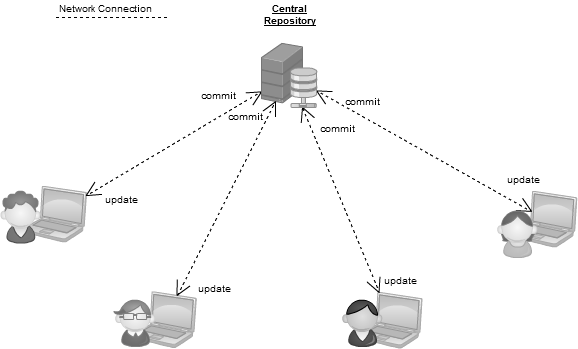
\includegraphics[width=0.75\textwidth]{CVCS.png}\caption{Visar upplägget i ett centraliserat versionshanteringssytem. Alla användare kopplar upp sig mot ett gemensamt repo}\label{fig:CVCSPic}\end{figure}



Datavetenskapsinstitutionen har valt att lära ut ett VCS kallat Concurrent Versions System (CVS) till PVG-projektet. CVS lanserades år 1990 och är ett centraliserat VCS (CVCS). Att det är centraliserat innebär att det har ett centralt repo som alla utvecklare kopplar upp sig mot (se Fig.~\ref{fig:CVCSPic}). I repot finns alla filer samt information om alla ändringar som gjorts. När en utvecklare checkar ut projektet skapas en lokal kopia av det på utveklarens dator. Därefter görs alla ändringar lokalt och när koden är klar laddar utvecklaren upp den i repot och löser eventuella merge-konflikter. Skulle ny kod bli uppladdat på repot går det att göra en uppdatering och på så sätt få de senaste ändringarna i sitt lokala repo. Allt detta kan göras via ett inbyggt användargränssnitt(GUI) i Eclipse. 

	CVS utvecklas inte längre men det finns många CVS-kloner som har samma funktionalitet som CVS. Klonerna är främst utvecklade för att lösa buggar och lägga till funktioner som saknades i den sista släppta versionen av CVS. Subversion (SVN) är en av dessa kloner och är systemet som används under PVG-projekten. Funktionerna som finns i CVS finns även i SVN och fungerar analogt. Även för SVN finns det GUI att installera till Eclipse för att grafiskt hantera projektfilerna. 
 

\subsection{Git}

\begin{figure}[htb!]\centering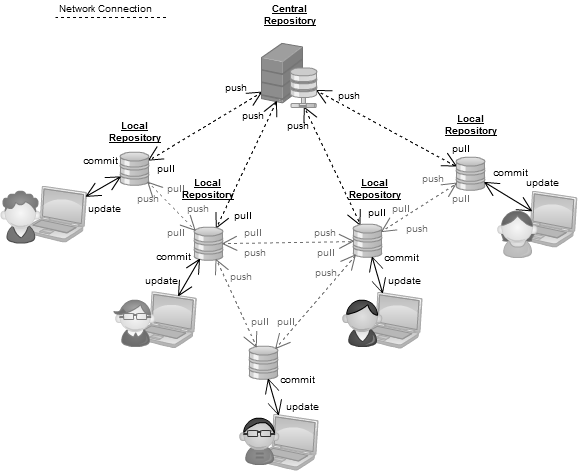
\includegraphics[width=0.75\textwidth]{DVCS.png}\caption{Visar upplägget i ett decentraliserat versionshanteringssytem. Alla användare kan koppla upp sig mot ett centralt repo men kan också dela filer mellan varandra}\label{fig:DVCSPic}\end{figure}


För att hantera källkoden till Linuxkärnan valde Linus Torvalds att utveckla sitt eget system~\cite{Torvalds}. Tidigare hade ett system kallat BitKeeper används men när projektets gratislicens gick ut behövdes ett nytt gratis VCS. Enligt Torvalds kunde inget av de dåvarande gratisalternativen leverera den funktionalitet som behövdes så han valde att istället utveckla sitt eget. Det beslutet resulterade i Git.

Till skillnad från CVS och SVN är Git ett decentraliserat VCS(DVCS). Detta innebär att det inte finns ett gemensamt repo som alla utvecklare använder sig av. Istället delar utvecklarna filerna mellan sig (se Fig. \ref{fig:DVCSPic}). Alla utvecklare har ett eget lokalt repo med alla filer och all filhistorik och när man behöver den senaste versionen av koden hämtar man den från de andra utvecklarna. När en utvecklare själv har gjort ändringar kan han trycka ut den nya koden till de andra utvecklarna. Git kan även användas som ett centraliserat VCS genom att alla hämtar från och trycker upp uppdateringar på en server. En av fördelarna med ett decentraliserat system är att två personer kan arbeta med en del i projektet och dela experimentell kod mellan sig utan att det påverkar resten av teamet. 

	Arbetsflödet i Git påminner mycket om det som används i CVS/SVN. Man arbetar med det lokala repot på samma vis som man arbetar med ett repo i CVS/SVN. Varje gång man gjort ändringar i koden gör man en commit till det lokala repot. När koden är redo att skickas ut till de andra utvecklarna trycker man ut koden till dem, vilket kallas att göra en push. Genom att commita till sitt eget repo får man även lokalt en historik som är enkel att navigera i då man alltid kan återställa filerna till en tidigare commit.
	
	Git kan användas både genom terminaler och genom grafiska GUI. Det finns både plugins och fristående program för att hantera sitt repo. Med installationen av Git medföljer även två simpla GUI som kan användas för att skapa och hantera branchar. Till Eclipse finns pluginet EGit vilket medför att man kan hantera sitt repo inifrån Eclipse.

%Bakgrund of the chosen area: summary of the chosen area. The purpose is to describe why, how and
%for which purpose the area is used.

%In this section quality will be defined in regard to both code quality and product quality. It will also describe why and how Test Driven Development, TDD, improves the quality of a product as well as the purpose of using TDD.

\section{Utförande} 
\label{utforande}
\subsection{Upplägg}
\label{Upplagg}

\begin{figure}[htb!]\centering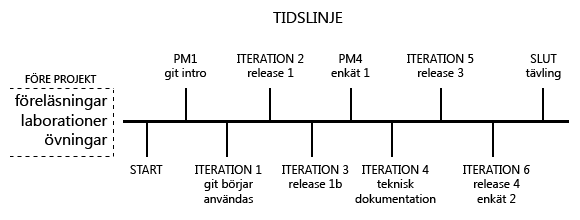
\includegraphics[width=0.75\textwidth]{Tidslinje.png}\caption{Visar tidsupplägget i projektet med viktiga händelser (PM = Planeringsmöte)}\label{fig:Timeline}\end{figure}

Vi lade upp arbete så att vi inte skulle lägga för mycket fokus på att använda Git som VCS då det är mycket ny information. Vårt team som vi skulle utbilda har inte varit i någon kontakt med Git innan men har inte heller några djuprotade arbetsätt med något annat versionhanteringssystem. Vi har delat upp upplägget för gruppen i tre faser. Första fasen är rent teoretisk och vi försöker hålla den på så grundläggande nivå som möjligt. Vi måste ständigt hålla i åtanke att för de flesta i gruppen som vi introducerar Git till har aldrig arbetat med något projekt av denna storlek innan. Detta innebär att de har fullt upp med mycket annat och ger vi dem för mycket teori så kommer den ändå inte befästas. Gruppen har redan en god insikt till vikten av att kunna arbeta parallellt och vill lära sig mer om det. 

Då vi också var nya till Git bara någon månad tidigare så förstår vi deras situation och har lättare för att skriva ner en kort guide på de mest nödvändigaste kommandona för att kunna arbeta med vårt projekt [Appendix A]. Denna guide delar vi ut på första planeringsmötet så alla kan direkt komma igång med att klona ner och arbeta med koden på första långlabben. Vi tilldelar även en i gruppen att läsa på mer teori och även testa lite själv, på så vis har de en VCS expert inom gruppen då det kan kännas lättare att prata med varandra.
 
Fas två uppstår vid första labben och för det flesta är därmed deras mer teoretiska lärande färdigt. Här efter kommer de uteslutande lära sig av vad de ser och gör. Det vill säga att de ser vilka fördelar Git har och i vilka situationer man använder sig av olika funktioner. I fas två är gruppen fortfarande väldigt outbildad vilket leder till att vi coacher går runt och hjälper dem vid mer komplicerade kommandon och händelser. Till att börja med så behöver de inte lära sig dessa alls utan bara kunna det som gavs till dem i fas ett. Allt efter som så får de själva skriva in kommandona och vi står bakom och instruerar och bara kontrollerar så att allt görs rätt. Vissa i gruppen som inte vill lära sig så mycket om Git kommer stanna i denna fas.

Efter några veckor av labbande kommer fler och fler i gruppen att ta till sig arbets sättet och inte tillkalla oss då de redan vet vilka kommandon som ska skrivas. De är då som fas tre inleds med mycket mer självgående användande utav Git. De vet själva vad som ska göras och kommer själva med förslag när de vill brancha för att till exempel arbeta i tätt samarbete med en annan grupp för att uppnå ett bättre resultat snabbare. För sådana strukturella beslut som att det går snabbare att två grupper branchar ut och arbetar tillsammans godkänner vi det först, men inte för att de inte tekniskt klarar det utan att vi fortfarande kan utvärdera om det finns någon vinning i att göra det.

Det är för det mesta väldigt säkert att låta grupperna själva experimentera själva så fort de har lärt sig grunderna eftersom Git är väldigt robust och man kan nästan alltid återskapa det mesta.

Detta speciellt då vi har minst fem stycken lokala repon med komplett historik samt en server. Följer de även den utdelade guiden och ofta commitar upp till sina egna lokala repon så kan man återställa nästan alla fel.

\subsection{Planeringsmöten}

I slutet av varje långlabb ska studenterna skriva ett par meningar om den specifika XP practice som de har fokuserat på. Vi har även lagt till att de också ska skriva om saker och ting som går bra och mindre bra med gruppen och vårt arbete, där vi belyst att om det är några problem med Git så ska de gärna ta upp dem här då vi coacher lättare kan ta tag och åtgärda dem. Dessa punkter tas sedan upp på våra schemalagda planeringsmöten för diskussion och reflektion. Vi kommer här med förslag till lösningar på hur vi ska åtgärda dessa och om någon i gruppen har något sätt. Här ser vi om vi till exempel skulle behöva skriva en ytterligare guide för att sätta in gruppen i de lite svårare funktionerna eller om de kan lära sig dem som beskrivet ovan i \ref{Upplagg} 

I slutet av planeringsmötena delar vi ut spikes till studenterna och om det har varit något som flera har uppfattat som svårt eller problematiskt inom Git så sprider vi kunskapen genom att någon gör ett grundligare undersökning varför det blev så och hur vi ska göra i fortsättningen. För det absolut mesta så vet vi coacher redan detta men  vi trycker hårt på att teamet ska besitta all kunskap själva och inte vara beroende utav oss coacher. Det kan även förekomma flera tillfällen då gruppen tycker att det är lättare eller smidigare att fråga varandra istället för oss coacher.

Det är viktigt att vi alla i gruppen också ska kunna ha tillgång till koden hemma för att kunna göra eventuella spikes så som till exempel kod granskning eller undersöka förslag till hur det är bäst att vidare utveckla en viss gren av programmet. För att detta ska fungera så har vi skrivit ihop en kort guide på den gemensamma trac-hemsidan. Där har vi också lagt upp ett shell-script som konfigurerar Git till deras inställningar utan att studenterna själva behöver skriva några kommandon.

Under de senare veckorna då gruppen arbetar mer självständigt med Git så skapar vi brancher även för de spikes som kräver något ur repot men även ska uppdatera repot till en ny version. Ledningen av kursen har beslutat att det får inte skrivas någon kod som trycks upp i repot mellan långlabbarna men gruppen får till exempel uppdatera JavaDoc eller teknisk dokumentation Det är viktigt för oss att dessa spikes inte blir för många och att de inte jobbar direkt på vår huvudbranch (master) utan att vi innan långlabben börjar kan merga ihop brancherna. Dessa merges ska alltid gå automatiskt då det inte ska vara flera brancher med samma ändringar. Till exempel så kan vi en vecka ha en spike med JavaDoc uppdateringar och en spike med att uppdatera manualen. Dessa två blir brancher för att kunna arbeta hemifrån utan att störa folk som vill ladda ner koden och få en halvt färdig skriven JavaDoc eller manual. Direkt då långlabben startar tar man en utav brancherna och mergar ihop den med master. Detta blir i git endast en fast forward och inga merge konflikter då det är bara en person som har ändrat. Sedan går vi till den andra spiken och gör det samma. Git löser denna merge-konflikten automatiskt då den tekniska dokumentationen inte har gjort några ändringar i några Java-filer och JavaDocen inte ska ha gjort några ändringar i den tekniska dokumentationen.

Ledningen för kursen har även godkänt att större refaktoriseringar utav hela programmet arkitekt kan vara bra att göra hemma då det förövrigt är produktionsstop då det annars skulle bli väldigt stora och svåra merge konflikter. När vi har dessa spikes är det viktigt att den spikegruppen är den ända som arbetar med koden och att alla har en god förståelse på vilka ändringar som kommer att göras och hur systemet kommer att se ut efteråt. Det är viktigt att lägga detta arbete på en egen branch då arbetet kan göras stegvis med flera commits under tiden. Att göra refaktoriseringar stegvis är inte bara bra för att andra får lättare att integrera sin kod utan att man lättare själv kan gå tillbaka om något inte blir bra. En annan mycket viktig aspekt på varför refaktoriseringen inte får ske på huvudbranchen är om den inte skulle lyckas bli klar så ska det inte vara några problem och alla kan bara arbeta på som vanligt. Skulle refaktoriseringen sedan bli klar någon timme in under labben så kan man fortfarande merga ihop den då. Det medför dock att man måste vara noggrann med den funktionalitet som har tillkommit under tiden.

\subsection{Git-konfiguration}

Git är mycket fritt och kan användas på många olika sätt där ingen är bunden att ställa sig i en hierarki. Vi har dock valt att arbeta med Git på ett lättförståligt sätt där alla hämtar(pull) det senaste från en server. På detta vis löser vi det krångliga som kan uppstå med att hämta från flera håll. Alternativet skulle vara att när en grupp har blivit klar med en story så hämtar alla ner hans version och mergar ihop med sitt eget. Här blir det dock lite rörigt i vår situation då vi enligt XP anda gör par byten och det slutar snabbt med att man inte har någon aning om vilken dator och inloggning man sitter på. Ett annat vanligt sätt att arbeta på är att ha en så kallad Gatekeeper~\cite{Gatekeeper} som alla hämtar ifrån. När ett par av utvecklare är färdiga med en story så säger man till Gate keepern som då hämtar från deras, kontrollerar ändringarna och kanske testkör programmet. När han är nöjd säger han till alla att det finns en ny version hos honom som alla ska hämta. Detta sättet är för visso mer säkert och röd kod sprider sig inte när någon har gjort fel. Dock så tycker vi coacher att detta inte känns så agilt och den snabbheten som är så viktig går lite förlorad. Det betyder även att teamet är beroende av denna enda “bättre vetande” personen som skall granska alla arbeten, vilket vi inte heller tycker går helt enligt XP. Vi vill med vår grupp uppnå en väldigt självgående sammansättning där vi coacher inte ska ha någon avgörande roll, och vi vill även att gruppen ska fungera vi eventuella bortfall. 
Vi har därför valt det upplägget som vi har och delar istället ut en task på att något annat utvecklingspar granskar en story innan den anses helt färdig. 


\subsection{Enkätundersökning}

För att mer konkret kunna analysera vår utvekling och ge oss feedback om hur bra matrialet och vår undervisning är så har vi lämnat ut en enkät [Appendix B]. I enkäten försöker vi adressera de olika faserna och se hur framgångsrika de har varit. Vi har ställt enkla frågor för att se hur lätt det var att ta till sig teorin i fas ett. Att komma igång med ett naturligt arbetsflöde i fas två. Vi undersöker huruvida de känner sig bekväma med Git och får djupare försåelse för det genom terminalen i steg tre, samt hurvida de skulle kunna tänka sig att arbeta med det i framtiden för en eventuellt fas fyra. Vi ger ut enkäten två gånger under kursens gång för att kunna analysera några förändringar. Den första gången är efter cirka halva tiden då de flesta i gruppen är i mitten eller slutet av fas två och den andra gången vi undersöker är på sista mötet då allt arbete med Git ska vara avklarat. 	

\section{Resultat}
\label{resultat}
Här följer de resultat som vi har som vi samlat in under studien. De innehåller dels resultaten från den enkät som delas ut vid två tillfällen till gruppen. Vi tar även upp våra egna observationer över hur inlärningen har utvecklats med tiden. 

\subsection{GIT i AGILA UTVECKLINGSPROJEKT}
Av de observationer som vi har kunnat göra iform utav coacher har vi kommit framtill att vi ser tydliga framsteg både i förståelsen för hur ett projekt av större storlek fungerar och vilka nya problem som uppstår. Framför allt så har vi observerat att studenterna ser stor nytta av ett versionshatneringssystem och den gemensamma uppfattningen är att Git fungerar väldigt bra. Vi själva tycker att problemen kring verktyget är få och förhållande små. Då vi pratar med andra grupper, som läser samma kurs, så framgår det tydligt att vi har mycket mindre problem. Detta tror vi dels för att Git har mycket bättre merge-vertyg och att vi inte använder oss utav något eclipse plugin. Eftersom vi använder git i terminalen får vi även en effekt av att man tänker till en extra gång innan man gör något. Vi tror att det är bra och tror inte att det leder till att man sprider sin kod mer sällan utan att utvecklarna tänker till innan och inte sprider felaktig kod lika ofta. 

Vi ser att git växer mer och mer i de framtidsrapport vi har studerat och en intressant tanke för kursen skulle vara att ersätta CVS/SVN med Git. Gruppen utvecklar i Eclipse som IDE, och den senaste versionen av programmet kommer med en mycket uppskattad version av EGit/JGit. Vi coacher har testat detta och ser fördelarna med att använda ett grafiskt plugin för att underlätta för utvecklarna. Den förberedande laborationen, se figur \ref{fig:Timeline} , skulle då inrikta sig på att lära ut Egit. Problemet på denna lösning är att Instutitionen förnärvarande endast levererar en Eclipse version som är två versioner bakom. 

\subsection{UTVECKLING}
\subsection{ENKÄTUNDERSÖKNING}
Här följer de frågor som fanns med i enkäten som delades ut samt en kort diskussion om resultaten.

\subsubsection{Snabbguiden gjorde det enkelt att förstå grunderna i Git}

\subsubsection{Det är lätt att få igång ett bra workflow (liknande update, update, update, commit för SVN)}


\subsubsection{Att använda Terminalen gör att man förstår bättre hur Git fungerar}


\subsubsection{Git hanterar mergkonflikter på ett bra sätt}


\subsubsection{Git fungerar bra tillsammans med Eclipse}


\subsubsection{När vi stöter på problem med Git kan ni som coacher ofta lösa det}


\subsubsection{Mitt helhetsintryck av Git är att det är ett bra versionshanteringssystem}


\subsubsection{Jag kommer fortsätta använda Git som versionshanteringssystem}


\section{Slutsats}
\label{slutsats}
Vi har under denna kurs och studie kommit fram till att Git fungerar utmärkt som versionshanteringssystem i agila utveklingsmiljöer. Vi har också fastslagit att det är möjligt att introducera Git, om även på ett mycket grundläggande plan, till en grupp studenter tillika utvecklare som aldrig arbetat med det innan. Verktyget har överlag fått god till mycket god kritik av gruppen. Vi visar härmed att Git skulle vara ett bättre alternativ än nuvarande SVN för kursen med bättre framtidsutsikter vilket är viktigt för blivande Civilingenjörer.  

\section{Terminologi}
\label{terminologi}
\begin{table}

\begin{tabular}{ | l |  p{7cm} |}
\hline
\emph{Uttryck}	 & \emph{Betydelse} \\ \hline \hline \\
Versionshanteringssystem (VCS) &	System som hanterar historik för källkod och dokument. \\ \hline 
 \\Repositorie (Repo) &	Server där projektets dokument, filer och historik lagras. \\ \hline 
 \\ Merge	& När man slår ihop två versioner av samma dokument eller fil. \\ \hline 
\\Branch & En kopia av projektet som utvecklas för sig själv, parallellt med projektet.  \\ \hline
\\Centraliserat VCS (CVCS) &	VCS där alla utvecklare kopplar upp sig mot ett gemensamt repositorie. \\ \hline
\\Decentralisert VCS (DVCS) &	VCS där alla utvecklare kan välja att koppla upp sig mot ett gemensamt repositorie eller att dela projektfiler mellan sig. \\ \hline
\\Concurrent Versions System (CVS) &	Är ett centraliserat VCS som idag inte utvecklas längre. \\ \hline
\\Subversion (SVN) &	System som bygger på CVS men som fortfarande utvecklas aktivt. \\ \hline
\\Git &	Är ett decentraliserat VCS. \\ \hline
\\Java &	Är ett programmeringsspråk som används i studien. \\ \hline
\\Commit &	Termen i CVS/SVN för när en utvecklare har ändrat i en fil och lägger upp ändringen i VCS. \\ \hline
\\Push &	Term för när en utvecklare som använder Git trycker ut sitt repositorie till andra utvecklare. \\ \hline
\\Update &	Används i CVS/SVN när en utevecklare hämtar hem de senaste versionerna av projektet. \\ \hline
\\Pull	 & Samma som Update för CVS/SVN men för Git. \\ \hline
\\eXtreme Programming (XP) &	Utvecklingsmetod framtagen av Kent Beck. \\ \hline
\\Story &	När en funktion ska utvecklas i XP skrivs denna som en story som beskriver vad som ska göras. \\ \hline
\\Task	& När en story delas upp i mindre problem blir dessa tasks. \\ \hline
\\Spike &	Egentid för att experimentera fram lösningar eller ideer. \\ \hline
\\Refaktorisering &	När kod förenklas och förbättras genom att minska komplexitet och göra saker mer tydliga. \\ \hline
\\Gate Keeper &	Vid användande av Git kan alla nya ändringar skickas till en person som granskar och därefter godkänner eller avslår ändringarna.  \\ \hline
\\JavaDoc &	Dokumentation som beskriver en Java-klass och alla dess publika metoder. \\ \hline
\\JUnit	& Program som kan användas för att skriva enhetstester för Java-program. \\ \hline
\\Trac	& En Wiki hemsida som gruppen använder för att strukturera sitt arbete. \\ \hline
\\Fast-forward & Git uppdatera till en ny version med ändringar från bara ett ställe och inga konflikter. \\ \hline

\end{tabular}
\end{table}




% needed in second column of first page if using \IEEEpubid
%\IEEEpubidadjcol

%\subsubsection{Subsubsection Heading Here}
%Subsubsection text here.


% An example of a floating figure using the graphicx package.
% Note that \label must occur AFTER (or within) \caption.
% For figures, \caption should occur after the \includegraphics.
% Note that IEEEtran v1.7 and later has special internal code that
% is designed to preserve the operation of \label within \caption
% even when the captionsoff option is in effect. However, because
% of issues like this, it may be the safest practice to put all your
% \label just after \caption rather than within \caption{}.
%
% Reminder: the "draftcls" or "draftclsnofoot", not "draft", class
% option should be used if it is desired that the figures are to be
% displayed while in draft mode.
%
%\begin{figure}[!t]
%\centering
%\includegraphics[width=2.5in]{myfigure}
% where an .eps filename suffix will be assumed under latex, 
% and a .pdf suffix will be assumed for pdflatex; or what has been declared
% via \DeclareGraphicsExtensions.
%\caption{Simulation Results}
%\label{fig_sim}
%\end{figure}

% Note that IEEE typically puts floats only at the top, even when this
% results in a large percentage of a column being occupied by floats.
% However, the Computer Society has been known to put floats at the bottom.


% An example of a double column floating figure using two subfigures.
% (The subfig.sty package must be loaded for this to work.)
% The subfigure \label commands are set within each subfloat command, the
% \label for the overall figure must come after \caption.
% \hfil must be used as a separator to get equal spacing.
% The subfigure.sty package works much the same way, except \subfigure is
% used instead of \subfloat.
%
%\begin{figure*}[!t]
%\centerline{\subfloat[Case I]\includegraphics[width=2.5in]{subfigcase1}%
%\label{fig_first_case}}
%\hfil
%\subfloat[Case II]{\includegraphics[width=2.5in]{subfigcase2}%
%\label{fig_second_case}}}
%\caption{Simulation results}
%\label{fig_sim}
%\end{figure*}
%
% Note that often IEEE papers with subfigures do not employ subfigure
% captions (using the optional argument to \subfloat), but instead will
% reference/describe all of them (a), (b), etc., within the main caption.


% An example of a floating table. Note that, for IEEE style tables, the 
% \caption command should come BEFORE the table. Table text will default to
% \footnotesize as IEEE normally uses this smaller font for tables.
% The \label must come after \caption as always.
%
%\begin{table}[!t]
%% increase table row spacing, adjust to taste
%\renewcommand{\arraystretch}{1.3}
% if using array.sty, it might be a good idea to tweak the value of
% \extrarowheight as needed to properly center the text within the cells
%\caption{An Example of a Table}
%\label{table_example}
%\centering
%% Some packages, such as MDW tools, offer better commands for making tables
%% than the plain LaTeX2e tabular which is used here.
%\begin{tabular}{|c||c|}
%\hline
%One & Two\\
%\hline
%Three & Four\\
%\hline
%\end{tabular}
%\end{table}


% Note that IEEE does not put floats in the very first column - or typically
% anywhere on the first page for that matter. Also, in-text middle ("here")
% positioning is not used. Most IEEE journals use top floats exclusively.
% However, Computer Society journals sometimes do use bottom floats - bear
% this in mind when choosing appropriate optional arguments for the
% figure/table environments.
% Note that, LaTeX2e, unlike IEEE journals, places footnotes above bottom
% floats. This can be corrected via the \fnbelowfloat command of the
% stfloats package.







% if have a single appendix:
%\appendix[Proof of the Zonklar Equations]
% or
\newpage
\appendix  % for no appendix heading
% do not use \section anymore after \appendix, only \section*
% is possibly needed

\appendices

\input{enkat}
\input{gitguide}


% use appendices with more than one appendix
% then use \section to start each appendix
% you must declare a \section before using any
% \subsection or using \label (\appendices by itself
% starts a section numbered zero.)
%


%\appendices
%\ection{Proof of the First Zonklar Equation}
%Appendix one text goes here.

% you can choose not to have a title for an appendix
% if you want by leaving the argument blank
%\ection{}
%Appendix two text goes here.



% Can use something like this to put references on a page
% by themselves when using endfloat and the captionsoff option.
\ifCLASSOPTIONcaptionsoff
  \newpage
\fi



% trigger a \newpage just before the given reference
% number - used to balance the columns on the last page
% adjust value as needed - may need to be readjusted if
% the document is modified later
%\IEEEtriggeratref{8}
% The "triggered" command can be changed if desired:
%\IEEEtriggercmd{\enlargethispage{-5in}}

% references section

% can use a bibliography generated by BibTeX as a .bbl file
% BibTeX documentation can be easily obtained at:
% http://www.ctan.org/tex-archive/biblio/bibtex/contrib/doc/
% The IEEEtran BibTeX style support page is at:
% http://www.michaelshell.org/tex/ieeetran/bibtex/
%\bibliographystyle{IEEEtran}
% argument is your BibTeX string definitions and bibliography database(s)
%\bibliography{IEEEabrv,../bib/paper}
%
% <OR> manually copy in the resultant .bbl file
% set second argument of \begin to the number of references
% (used to reserve space for the reference number labels box)
\newpage
\begin{thebibliography}{1}
\label{bibliography}



%\bibitem{IEEEhowto:kopka} % Add referenses in the same way as this one, and call them by ~\cite{biblabel}
%H.~Kopka and P.~W. Daly, \emph{A Guide to {\LaTeX}}, 3rd~ed.\hskip 1em plus
  %0.5em minus 0.4em\relax Harlow, England: Addison-Wesley, 1999.
 \bibitem{Browser}
Browser Statistics. W3Schools.com. \url{http://www.w3schools.com/browsers/browsers_stats.asp.}(February 2012)

 \bibitem{OpenSource}
Open Source Developer Preferences Survey. Microsoft Developer Network (MSDN). \url{http://blogs.msdn.com/b/codeplex/archive/2011/07/11/survey-results-open-source-developer-preferences-june-2011.aspx} (June 2011)

\bibitem{BeckTDD}
Beck, K., \emph{Test Driven Development -- by Example}. Boston: Addison Wesley, 2003.

\bibitem{BeckXP}
Beck, K., \emph{Extreme Programming Explained: Embrace Change}. Reading, Massachusetts: Addison-Wesley, 2000.

\bibitem{Torvalds}
McMillan, R. \emph{After controversy, Torvalds begins work on "git"}. \url{http://www.infoworld.com/t/platforms/after-controversy-torvalds-begins-work-git-721}. (April 2005)

\bibitem{Sullivan}
Bryan O'Sullivan. \emph{Making sense of revision-control systems}. Commun. ACM 52, 9. (September 2009)

\bibitem{Yip}
Yip, Chen \& Morris. \emph{Pastwatch: a Distributed Version Control System}. MIT Computer Science and AI Laboratory. (May 2006)
 
\bibitem{Mockus}
A. Mockus.\emph{Amassing and indexing a large sample of version control systems: Towards the census of public source code history}. Avaya Labs. Res. (May 2009)
 
\bibitem{Hedin}
Hedin, Bendix \& Magnusson. \emph{Teaching extreme programming to large groups of students}. Elsevier. (2005)

\bibitem{Asklund}
Asklund, Bendix \& Ekman. \emph{Software Configuration Management Praticies for eXtreme Programming Teams}. Department of Computer Science, Lund Institute of Technology. (August 2004)
 

  


\end{thebibliography}



% biography section
% 
% If you have an EPS/PDF photo (graphicx package needed) extra braces are
% needed around the contents of the optional argument to biography to prevent
% the LaTeX parser from getting confused when it sees the complicated
% \includegraphics command within an optional argument. (You could create
% your own custom macro containing the \includegraphics command to make things
% simpler here.)
%\begin{biography}[{\includegraphics[width=1in,height=1.25in,clip,keepaspectratio]{mshell}}]{Michael Shell}
% or if you just want to reserve a space for a photo:

%\begin{IEEEbiography}{Michael Shell}
%Biography text here.
%\end{IEEEbiography}
%
%% if you will not have a photo at all:
%\begin{IEEEbiographynophoto}{John Doe}
%Biography text here.
%\end{IEEEbiographynophoto}
%
%% insert where needed to balance the two columns on the last page with
%% biographies
%%\newpage
%
%\begin{IEEEbiographynophoto}{Jane Doe}
%Biography text here.
%\end{IEEEbiographynophoto}

% You can push biographies down or up by placing
% a \vfill before or after them. The appropriate
% use of \vfill depends on what kind of text is
% on the last page and whether or not the columns
% are being equalized.

%\vfill

% Can be used to pull up biographies so that the bottom of the last one
% is flush with the other column.
%\enlargethispage{-5in}



% that's all folks
\end{document}


